\newpage
\section{Aufbau und Durchführung}
\label{sec:Durchführung}
Der Aufbau des Versuchs ist in Abbildung \ref{fig:Versuch} zu erkennen.
Die Probe Kaliumbromid (\ce{KBr}), welche mit Strontiumionen (\ce{Sr}) hat eine Dicke von $d=\SI{3}{\milli\meter}$ und befindet sich auf dem Boden des Probebehälters.
Dieser wird durch die Vakuumpumpe auf \SI{e-2}{\milli\bar} evakuiert.
Die Probe wird für etwa \SI{15}{\minute} auf ungefähr \SI{320}{\kelvin} in einem angelegtem Feld von \SI{900}{\volt} erhitzt.
Um die Dipole "einzufrieren" wird die Probe durch flüssigen Stickstoff, über einen Kühlfinger auf ca \SI{210}{\kelvin} abgekühlt.
Der Kondensator wird kurzgeschlossen und für einige Minuten entladen.
Anschließend wird das Picoamperemeter angeklemmt und gewartet, dass sich ein konstanter Stromwert einstellt.
Es werden zwei Strom-Temperatur-Kurven bei einer konstanten Heizrate $h$ von \SI{2}{\kelvin\per\minute} und \SI{1}{\kelvin\per\minute} aufgenommen.
\begin{figure}[htb]
    \centering
    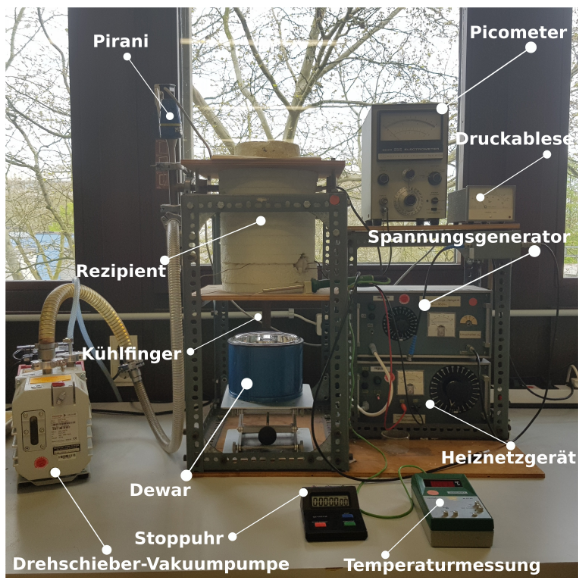
\includegraphics[height=8cm]{pics/Versuch.png}
    \caption{Der verwendete Versuchsaufbau. \cite{anleitung}}
    \label{fig:Versuch}
  \end{figure}
  \FloatBarrier